\documentclass[conference]{IEEEtran}
\IEEEoverridecommandlockouts
% The preceding line is only needed to identify funding in the first footnote. If that is unneeded, please comment it out.
\usepackage{cite}
\usepackage{amsmath,amssymb,amsfonts}
\usepackage{algorithmic}
\usepackage{graphicx}
\usepackage{hyperref}
\usepackage{textcomp}
\usepackage{xcolor}
\usepackage{listings}
\usepackage{lipsum}
\usepackage{eurosym}
\usepackage{soul}
\usepackage{color}

\DeclareRobustCommand{\hlcyan}[1]{{\sethlcolor{cyan}\hl{#1}}}

\colorlet{punct}{red!60!black}
\definecolor{background}{HTML}{EEEEEE}
\definecolor{delim}{RGB}{20,105,176}
\colorlet{numb}{blue!60!black}

\lstdefinelanguage{json}{
	basicstyle=\normalfont\ttfamily,
%	numbers=left,
%	numberstyle=\scriptsize,
%	stepnumber=1,
%	numbersep=8pt,
%	showstringspaces=false,
%	breaklines=true,
%	frame=lines,
%	backgroundcolor=\color{background},
	literate=
	*{0}{{{\color{numb}0}}}{1}
	{1}{{{\color{numb}1}}}{1}
	{2}{{{\color{numb}2}}}{1}
	{3}{{{\color{numb}3}}}{1}
	{4}{{{\color{numb}4}}}{1}
	{5}{{{\color{numb}5}}}{1}
	{6}{{{\color{numb}6}}}{1}
	{7}{{{\color{numb}7}}}{1}
	{8}{{{\color{numb}8}}}{1}
	{9}{{{\color{numb}9}}}{1}
	{:}{{{\color{punct}{:}}}}{1}
	{,}{{{\color{punct}{,}}}}{1}
	{\{}{{{\color{delim}{\{}}}}{1}
	{\}}{{{\color{delim}{\}}}}}{1}
	{[}{{{\color{delim}{[}}}}{1}
	{]}{{{\color{delim}{]}}}}{1},
}


\def\BibTeX{{\rm B\kern-.05em{\sc i\kern-.025em b}\kern-.08em
    T\kern-.1667em\lower.7ex\hbox{E}\kern-.125emX}}
\begin{document}

\title{ArduECO: Arduino based air quality control for shared transportation methods in cities}

\author{\IEEEauthorblockN{Voinea Stefan Ciprian}
\IEEEauthorblockA{\textit{University of Padova, Italy} \\
\textit{Department of Pure and Applied Mathematics}\\
	%Padova, Italy \\
	stefanciprian.voinea@studenti.unipd.it}
	%\and
	%\IEEEauthorblockN{2\textsuperscript{nd} Given Name Surname}
	%\IEEEauthorblockA{\textit{dept. name of organization (of Aff.)} \\
	%\textit{name of organization (of Aff.)}\\
	%City, Country \\
	%email address or ORCID}
}

\maketitle

%\begin{abstract}
%	\lipsum[1]
%\end{abstract}
%
%\vspace{.2cm}
%
%\begin{IEEEkeywords}
%Arduino, embedded, air-quality
%\end{IEEEkeywords}

\section{Introduction}\label{intro}
	More and more people around the world have started to understand the importance of air quality and how much having clean and pollution-free air can influence our lives, both on the small and large scale. 
	To have clean air, all of us have to do something to avoid polluting it. \\
	The Government of Luxembourg has set a good example, becoming the first country to offer nationwide free public transport to citizens\cite{luxemburg}.\\
	For short commutes, vehicles like the classic bike\cite{bike}, the infamous skateboard and the scooter have started to arise and conquer cities, either in their battery-powered or old-school human-powered form.\\
	Since not everyone necessarily owns one of these green methods of transportation, companies like \textit{Mobike}\cite{mobike} and \textit{MiMoto}\cite{mimoto} have seen the opportunity to enter the market of shared transportation, proposing a \textit{pay-per-use} solution for bikes, electric scooters and other similar vehicles.	
	Each company has its own phone application, network infrastructure and smart devices aboard their vehicles, gathering data like GPS (Global Positioning System) position, time spent by the user, parking spot, etc. to send it in the cloud and compute information like cost of the ride and charging it to the customer.\\
	All this falls under the \textit{IoT} (Internet of Things) paradigm, which has become a well-described market with new ideas and business opportunities being presented every day.\\
	Among the data collected by these companies, none is about air pollution.\\
	This article describes \textit{ArduECO}, a wireless device based on an Arduino-like board capable of gathering data about air quality (and more) from previously named vehicles and sending it to the cloud, to be processed and displayed.\\
	This paper is organized as follows:
	\begin{itemize}
		\item Section \ref{bck}: description of the problem that this essay aims to solve and state of the art on smart devices that allow tracking pollution;
		\item Section \ref{solution}: how ArduECO has been implemented;
		\item Section \ref{improvements}: improvements to this project;
		\item Section \ref{conclusions}: conclusions.
	\end{itemize}

\section{Background problem and state of the art}\label{bck}
	Tracking air quality is an important task usually tied to weather agencies involving trucks seen parked or going around the city, collecting data like \textit{PM 2.5} and \textit{PM 10}.\\
	\textit{PM} stands for \textit{Particulate Matter} and indicates the term for a mixture of solid particles and liquid droplets found in the air, with diameters around 2.5 or 10 micrometers.
	Some particles, such as dust, dirt, soot, or smoke, are large or dark enough to be seen with the naked eye, others can only be detected using an electron microscope\cite{particles}.\\
	In cities like Padova and Milan\cite{milano}, a great percentage of PM production has been cut by decreasing the number of cars that can circulate and introducing more ways of public transportation: for example pay-per-use bike services have seen in the last year a vast amount of users.
	Fig.~\ref{mobi} is an infographic released by Mobike that shows the amount of CO2 emissions in Kg spared during 2019 by using their shared bikes.
	\begin{figure}[htbp]
		\centerline{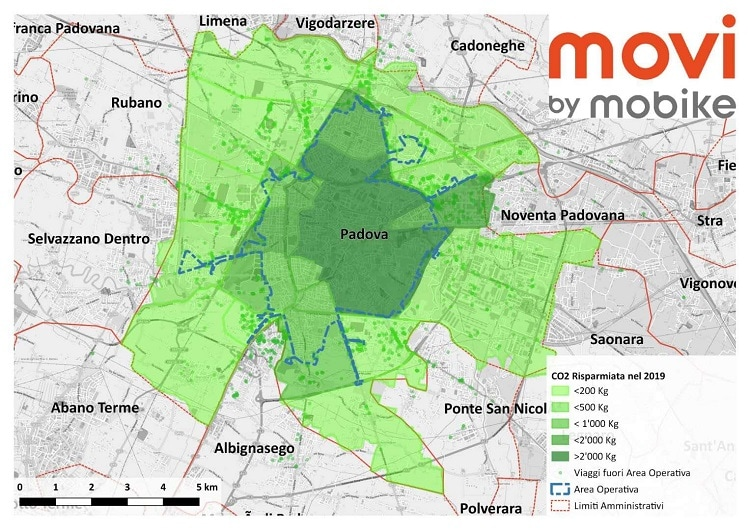
\includegraphics[width=8.8cm]{fig3.jpg}}
		\caption{Example of a figure caption.\cite{mobike_pd}}
		\label{mobi}
	\end{figure}\\
	Since Mobike's launch in Padova in 2019, its users have biked over 330.000 Km across the city and reduced CO{\footnotesize 2} emissions by over 60 tons.\\
	CO (Carbon Monoxide) and CO{\footnotesize 2} (Carbon Dioxide) are gasses that become important pollutants when associated with cars, planes, power plants, and other human activities that involve the burning of fossil fuels such as gasoline and natural gas\cite{co2}.\\
	There have been various attempts to create portable gas detectors, both for academic and marketing purposes.
	In 2014 Cambridge University proposed hand-held devices with electro-chemical sensors inside to collect and store data or send it in real time to a central computer for analysis\cite{cambridge}.
	Researches like these generally tend to remain limited in the academic field.
	\textit{Flow}\cite{flow}, on the other hand, is a device with similar capabilities of the one from Cambridge, only that it's proprietary and sold on the market to consumers interested in their personal well-being.\\
	These devices are usually implemented using \textit{low-cost} sensors like the ones in MQ-series, made of a heating element an electro-chemical sensor, which will react only when it reaches certain temperatures.\\
	ArduECO has been designed using the \textit{MQ-7} sensor, sensible for \textit{Carbon Monoxide}.
	
\section{Proposed solution}\label{solution}
	
	ArduECO is a wireless IoT device that represents one of the possible combinations of open source hardware and software.
	This wireless device is able to detect the amount of CO air and send this value in the cloud over Wi-Fi, and, combined with data from other similar devices, detect the level of pollution in the air.\\
	The schematics for this project have been designed using Fritzing, a CAD (Computer-Aided Design) software for the design of electronics hardware\cite{fritzing} and can be seen in Fig.~\ref{schematics}.
	Both code and schematics for this device are available on the GitHub repository ``ArduECO''\cite{ardueco_git}.\\
	Schematics for other components can be easily found online from various sources and vendors: here, for example are the schematics for the MQ7 sensor from SparkFun\cite{spark_mq} and the NodeMCU\cite{node_scheme}.\\
	The goal is to have a device small enough to fit on any of previously mentioned shared transportation methods.
	ArduECO would represent a possible solution: for example it could fit under baskets of bikes and be powered by dynamos that already power the headlight and other circuitry which allow this transport to be connected with the vendor's cloud (for example Mobike).
	Given the modularity of ArduECO it's circuit can easily be adapted to fit other cases and forms.
	
	\subsection{The circuit}\label{circuit}
	
		ArduECO is composed by four main components:
		\begin{itemize}
			\item \textit{NodeMCU}: it's the hearts and brains of the device, this board is an open-source development kit based on the ESP8266 chip that allows for prototyping of IoT devices;
			\item \textit{MicroSD card reader}: these allow for collecting and keeping data cached for the current ride and permanently on a removable memory card;
			\item \textit{GPS sensor}: this allows for localizing the device, it has an onboard LED that blinks when it has established communication with the satellites;
			% AGGIUNGERE COSA RACCOGLIE ESATTAMENTE QUESTO SENSORE
			\item \textit{MQ sensor}: the MQ-7can easily be exchanged with other sensors that use the same board and connectors.
		\end{itemize}
		The other components, LEDs and button, are used as I/O for interacting with the user.\\
		In Section \ref{improvements} I explain how the project can be improved both in hardware and software.
		\begin{figure}[htbp]
			\centerline{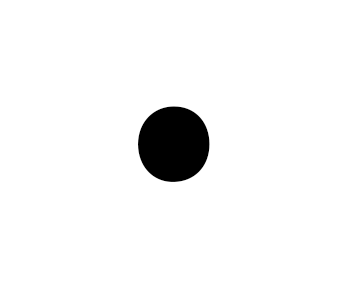
\includegraphics[width=8.8cm]{fig1.png}}
			\caption{ArduECO schematics}
			\label{schematics}
		\end{figure}
		In Fig.~\ref{schematics} there is no indication of a power supply since for this prototype version it has been powered using an external battery with a standard output of 5V and 1A.
	
	\subsection{The Arduino software}
	
		For ArduECO I chose to use Arduino's programming language instead of \cite{micropyhton} because of the large community supporting it and the vast interoperability with other boards.\\
		The main functions in the Arduino programming language are ``\textit{void setup()[]}'' and ``\textit{void loop()[]}'': the first one runs a single time when the device boots initializing and setting the initial values while the second one loops consecutively, allowing the program to change and respond.
		ArduECO.ino is the main file executed by the NodeMCU and contains the previously described functions.\\
		In ArduECO's software, the setup function contains the instructions to correctly initialize serial communication with the GPS module, create the files in the SD card, initialize the pin-outs, gather the certificates for communicating with the cloud and create a random id for identifying the ride, since each time the device boots is considered as a single ride.\\
		An important part of the configuration of ArduECO is the file \textit{params.json}:
		\begin{lstlisting}[language=json,firstnumber=1]
    {
	  "ssid" : "",
	  "password" : "",
	  "in_topic" : "",
	  "out_topic" : "",
	  "endpoint" : ""
    }
		\end{lstlisting}
		If this file is not present in the SD card at boot-time and correctly formatted, ArduECO will not end the boot sequence, returning an error and rebooting after 10 seconds.\\
		This file contains configurations such network SSID and password, topics for communicating with the MQTT server and its endpoint (network address).\\
		The loop function contains the instructions that tell the board to acquires a reading of its surroundings every 5 seconds by first detecting if a GPS fix if present and by reading the value from the analog pin connected to the MQ sensor.
		%TODO AGGIUNGERE FIGURA
		Each read is then appended on two separate text files (\textit{cache\_log.txt} and \textit{perm\_log.txt}) in JSON format. 
		\textit{cache\_log.txt} is created each time ArduECO boots is related to a single session while \textit{perm\_log.txt} contains reads about each ride taken.\\
		Here is an example of a logged loop cycle read:
		\begin{lstlisting}[language=json,firstnumber=1]		
    {
	  "id":"127",
	  "air":"18.22",
	  "lt":"45.39641",
	  "lg":"11.88527",
	  "dt":"50320.12173900",
	  "tpc":"ardueco_proto_01_OUT"
    }
		\end{lstlisting}	
		The external LEDs are used to communicate when the setup sequence has finished correctly with errors as well as for indicating whether the SSID specified in the \textit{params.json} file is in range and if ArduECO is transmitting data.\\
		When the button is pressed, ArduECO searches the list of networks in range for the specified one and, if present, connects to it.
		Afterwards it establishes communication with the MQTT server specified by the endpoint, and sending it a message with the number of messages that will be sent.\\
		Each row of the cache file is then transmitted to the server.\\
		At the end of this sequence the cache file is deleted and created again awaiting new reads.\\
		The other files that implement this project contain specific functions for either setting up the device or connecting the the server.
		
	\subsection{The cloud}
	
		When the button is pressed, ArduECO connects to the access point with the SSID specified in the \textit{params.json} file and sends the contents of \textit{cache\_log.txt} to the cloud, specifically to AWS (Amazon Web Services).
		\textit{IoT core} and \textit{Lambda} are the services that are used for this project.\\
		ArduECO sends data to the MQTT server in IoT core specified as \textit{endpoint} in \textit{params.js}.
		It connects to this server using certificates created in the IoT core console and that are loaded in ArduECO's memory, this means that they are uploaded via the Arduino IDE.\\
		The MQTT (Message Queuing Telemetry Transport) server is designed as a lightweight messaging protocol that uses publish/subscribe operations to exchange data between clients and server, fast in data transmission\cite{mqtt}.\\
		This service in IoT core is connected to a serveress Lambda function written in Python, triggered each time a new messages arrives from ArduECO, which receives the JSON message as a parameter and calls a PHP page on \href{ardueco.altervista.org}{ardueco.altervista.org}, where the front end of the service is hosted.
		Altervista is a free website hosting platform with PHP and MySQL database.
		After being saved in the MySQL database in Altervista is then displayed on the homepage using Google Maps' APIs.
		\begin{figure}[htbp]
			\centerline{\includegraphics[width=8.8cm]{fig2.png}}
			\caption{Map with markers and reads from \href{ardueco.altervista.org}{ArduECO}.}
			\label{altervista}
		\end{figure}
	
		Each marker on the map represents a reading and, if clicked on, shows the value read by ArduECO's sensor.\\
		Markers are connected with different colors indicating the ride they belong to.
		
	\subsection{Hardware cost}
	
		Because the components used for this project are open-source, they can be found sold on various websites from many vendors.
		Here are some examples of prices taken from the Chinese e-commerce AliExpress\cite{aliexpress} at the time of writing.
		\begin{itemize}
			\item NodeMCU \footnote{\url{https://it.aliexpress.com/item/32879925927.html}}: $ \sim $ 2\euro
			\item MicroSD car reader \footnote{\url{https://it.aliexpress.com/item/32572793362.html}}: $ \sim $ 0.50\euro
			\item GPS sensor \footnote{\url{https://it.aliexpress.com/item/32836015224.html}}: $ \sim $ 3.5\euro
			\item MQ gas sensor \footnote{\url{https://it.aliexpress.com/item/4000575957425.html}}: $ \sim $ 1\euro
		\end{itemize}
		The total cost of these items amounts to $\sim$ 7\euro, considering shipping and costs of remaining components (cables, LEDs, button, SD card), it can arrive to less than 15\euro.\\
		Note that the indicated prices refer to single pieces and in case of bulk purchases (at least 5 or 10 of each piece) the total cost would be much lower.
	
%\section{Results and data analysis}\label{data}
%	\hlcyan{DA FARE PER INTERO}
%	\subsection{Test scenarios}
%
%		\subsubsection{Prototype test}
%
%		\subsubsection{Real life implementation}
%			% \subsection{Abbreviations and Acronyms}\label{AA}
%			State of the art
%	
%	It make detection by method of cycle high and low temperature, and detect CO when low temperature \cite{mq7}


\section{Future improvements}\label{improvements}
	Since ArduECO is one of many possible implementations that this hardware and software can create, there are various improvements which could bring to a better and more stable device.
	
	\subsection{Hardware improvements}
		Many improvements can be made on the hardware: for example, the circuit described in Section \ref{circuit} has a single air sensor due to the limitation of the NodeMCU and ESP8266 chip that have only one analog input pin.\\
		By connecting the board to an \textit{ADC} (Analog to Digital Converter) it becomes possible to add multiple sensors expanding the analog inputs.
		ADCs convert an analog voltage on a pin to a digital number\cite{adc}.\\
		In order to upgrade the transmission method and use mobile data instead of WiFi (which is limited to 2.4GHz on the NodeMCU) it's possible to switch the board to an Arduino Leonardo or an Arduino Uno.\\
		Modules capable to add mobile connectivity can be found on sites like AliExpress\footnote{\href{https://it.aliexpress.com/item/32963853961.html}{https://it.aliexpress.com/item/32963853961.html}} and does not brig much additional overall cost (in this case $ \sim $ 2\euro).\\
		Given the small size of the components, this project could be easily fitted inside of a custom made box.
		A solution could be to design and 3D print a custom plastic case in which fit the whole device, considering that the air sensor should remain outside of the case and the whole project could be exposed to high levels of humidity (for example during the winter season).\\
		Powering is one important issue for IoT devices.
		The prototype described in this manuscript runs on an external battery, but it can be coupled with other energy sources like a dynamo, so that it can be powered by movement of the wheel (in case it's installed on a bike).
	
	\subsection{Software improvements}	
		The software can be improved in many ways as well.
		For example a control could be added to check if every message has correctly arrived at the IoT server and, in case of a timeout or an eventual error, the message could be sent again.\\
		In this project various libraries have been used for the Arduino sensors, a great improvement would be to better adapt these libraries for ArduECO, especially the MQ-7 library.\\
		Since this is an IoT device and battery is an essential need, adding a deep sleep mode could improve the performance of ArduECO.
		
	\subsection{Cloud services improvements}
		The cloud technologies can be improved too.
		AWS' IoT core could be configured to have more MQTT servers based on the groups of devices divided by each city or zone in which they're used.\\
		Another important change would be using an AWS EC2 instance to host the website instead of Altervista.\\
		Thinking about an architecture that could easily scale horizontally, and supporting more devices connected at once, the database can be switched from MySQL to Redis,  a NoSQL database that provides real-time and high-efficiency services for data storage, increasing the I/O speed by storing all key-value data in the memory\cite{redis}.\\
		These, thought, would introduce an expense for the AWS services, but offering high efficiency and modularity.\\
		Switching to these technologies would allow for a better Lambda function, directly connected to the database for example, as well.
		
\section{Conclusions and future work}\label{conclusions}

	Air pollution is an increasing problem on which many people and companies are working.\\
	In cities around the world shared methods of transportation like scooters and bikes have started to grow in popularity and the more people use them the better air quality gets in term of pollution released in the air.\\
	Centralized solutions are currently the most used to detect air pollution particles like PM 2.5, PM 10, CO and CO2, but they only collect data in their proximity.\\
	This essay describes the implementation of a PoC (Proof of Concept) wireless IoT device, ArduECO, capable to gather data from air, analyze and display it to the user.
	ArduECO uses an Arduino-like board (NodeMCU) with a built in WiFi to send data recorded from an MQ-7 sensor for CO and a GPS module, in the cloud.
	Here data is displayed on a map, with each marker indicating a reading from the device, as shown in Fig.~\ref{altervista}.\\
	As described in Section \ref{improvements} there are areas in which ArduECO can be improved, both in hardware and software, including a thorough data analysis.
	This could lead to the creation of a better platform which would allow each user of ArduECO to see his own ride, since this device is not intended to be standalone but to be spread out around the city.\\
	Companies like Mobike should be able to integrate their hardware with this devices without making excessive modifications to their existing bikes, scooter companies should be able to do so as well.\\
	With this kind of information people would be more actively stimulated to use shared green methods of transportation, knowing that by doing so their quality of life will get better in the near future.
		
\begin{thebibliography}{00}
	
\bibitem{luxemburg} \url{https://www.mobiliteit.lu/en/tickets/free-transport/}\\

\bibitem{b01} \url{https://www.wired.com/story/vehicle-future-bike/}\\

\bibitem{b02}  \href{https://www.ilsole24ore.com/art/in-bicicletta-lavoro-milano-risparmiate-275-tonnellate-co2-ACYBZ1FB}{https://www.ilsole24ore.com/art/in-bicicletta-lavoro-milano-risparmiate-275-tonnellate-co2-ACYBZ1FB}\\

\bibitem{b03} Official Arduino website: \url{https://www.arduino.cc/}\\

\bibitem{b04} Official Raspberry Pi website: \url{https://www.raspberrypi.org/}\\
	
\bibitem{b01} Lua based interactive firmware for ESP8266, ESP8285 and ESP32 \url{https://github.com/nodemcu/nodemcu-firmware}

http://www.padovaoggi.it/attualita/dati-mobike-padova-10-ottobre-2019.html

\bibitem{mobike} «In arrivo anche a Padova le E-Bike a pedalata assistita»: l'annuncio di Mobike
„«In arrivo anche a Padova le E-Bike a pedalata assistita»: l'annuncio di Mobike:  \href{http://www.padovaoggi.it/attualita/mobike-e-bike-dati-padova-21-febbraio-2020.html}{http://www.padovaoggi.it/attualita/mobike-e-bike-dati-padova-21-febbraio-2020.html}

https://arduinojson.org/
	
\bibitem{b20} G. Eason, B. Noble, and I. N. Sneddon, ``On certain integrals of Lipschitz-Hankel type involving products of Bessel functions,'' Phil. Trans. Roy. Soc. London, vol. A247, pp. 529--551, April 1955.
%\bibitem{b2} J. Clerk Maxwell, A Treatise on Electricity and Magnetism, 3rd ed., vol. 2. Oxford: Clarendon, 1892, pp.68--73.
%\bibitem{b3} I. S. Jacobs and C. P. Bean, ``Fine particles, thin films and exchange anisotropy,'' in Magnetism, vol. III, G. T. Rado and H. Suhl, Eds. New York: Academic, 1963, pp. 271--350.
%\bibitem{b4} K. Elissa, ``Title of paper if known,'' unpublished.
%\bibitem{b5} R. Nicole, ``Title of paper with only first word capitalized,'' J. Name Stand. Abbrev., in press.
%\bibitem{b6} Y. Yorozu, M. Hirano, K. Oka, and Y. Tagawa, ``Electron spectroscopy studies on magneto-optical media and plastic substrate interface,'' IEEE Transl. J. Magn. Japan, vol. 2, pp. 740--741, August 1987 [Digests 9th Annual Conf. Magnetics Japan, p. 301, 1982].
%\bibitem{b7} M. Young, The Technical Writer's Handbook. Mill Valley, CA: University Science, 1989.
\end{thebibliography}


\end{document}
